\documentclass[a4paper,notitlepage]{article}
\usepackage[utf8]{inputenc} %Make sure all UTF8 characters work in the document
\usepackage{listings} %Add code sections
\usepackage{color}
\usepackage[yyyymmdd]{datetime}
\usepackage{graphicx}
\usepackage{titling}
\usepackage{titlesec}
\usepackage{listliketab}
\usepackage{textcomp}
\usepackage[hyphens]{url}
\usepackage[bottom]{footmisc}
\definecolor{listinggray}{gray}{0.9}
\definecolor{lbcolor}{rgb}{0.9,0.9,0.9}
\usepackage{geometry}
\geometry{margin=3cm}
\usepackage{parskip} 

\hyphenation{regres-sions-test-er}

\renewcommand{\dateseparator}{--}
\renewcommand{\arraystretch}{1.3}
\titlespacing*\section{0pt}{10pt plus 4pt minus 2pt}{0pt plus 2pt minus 2pt}
\titlespacing*\subsection{0pt}{10pt plus 4pt minus 2pt}{0pt plus 2pt minus 2pt}
\pretitle{%
\begin{center}
	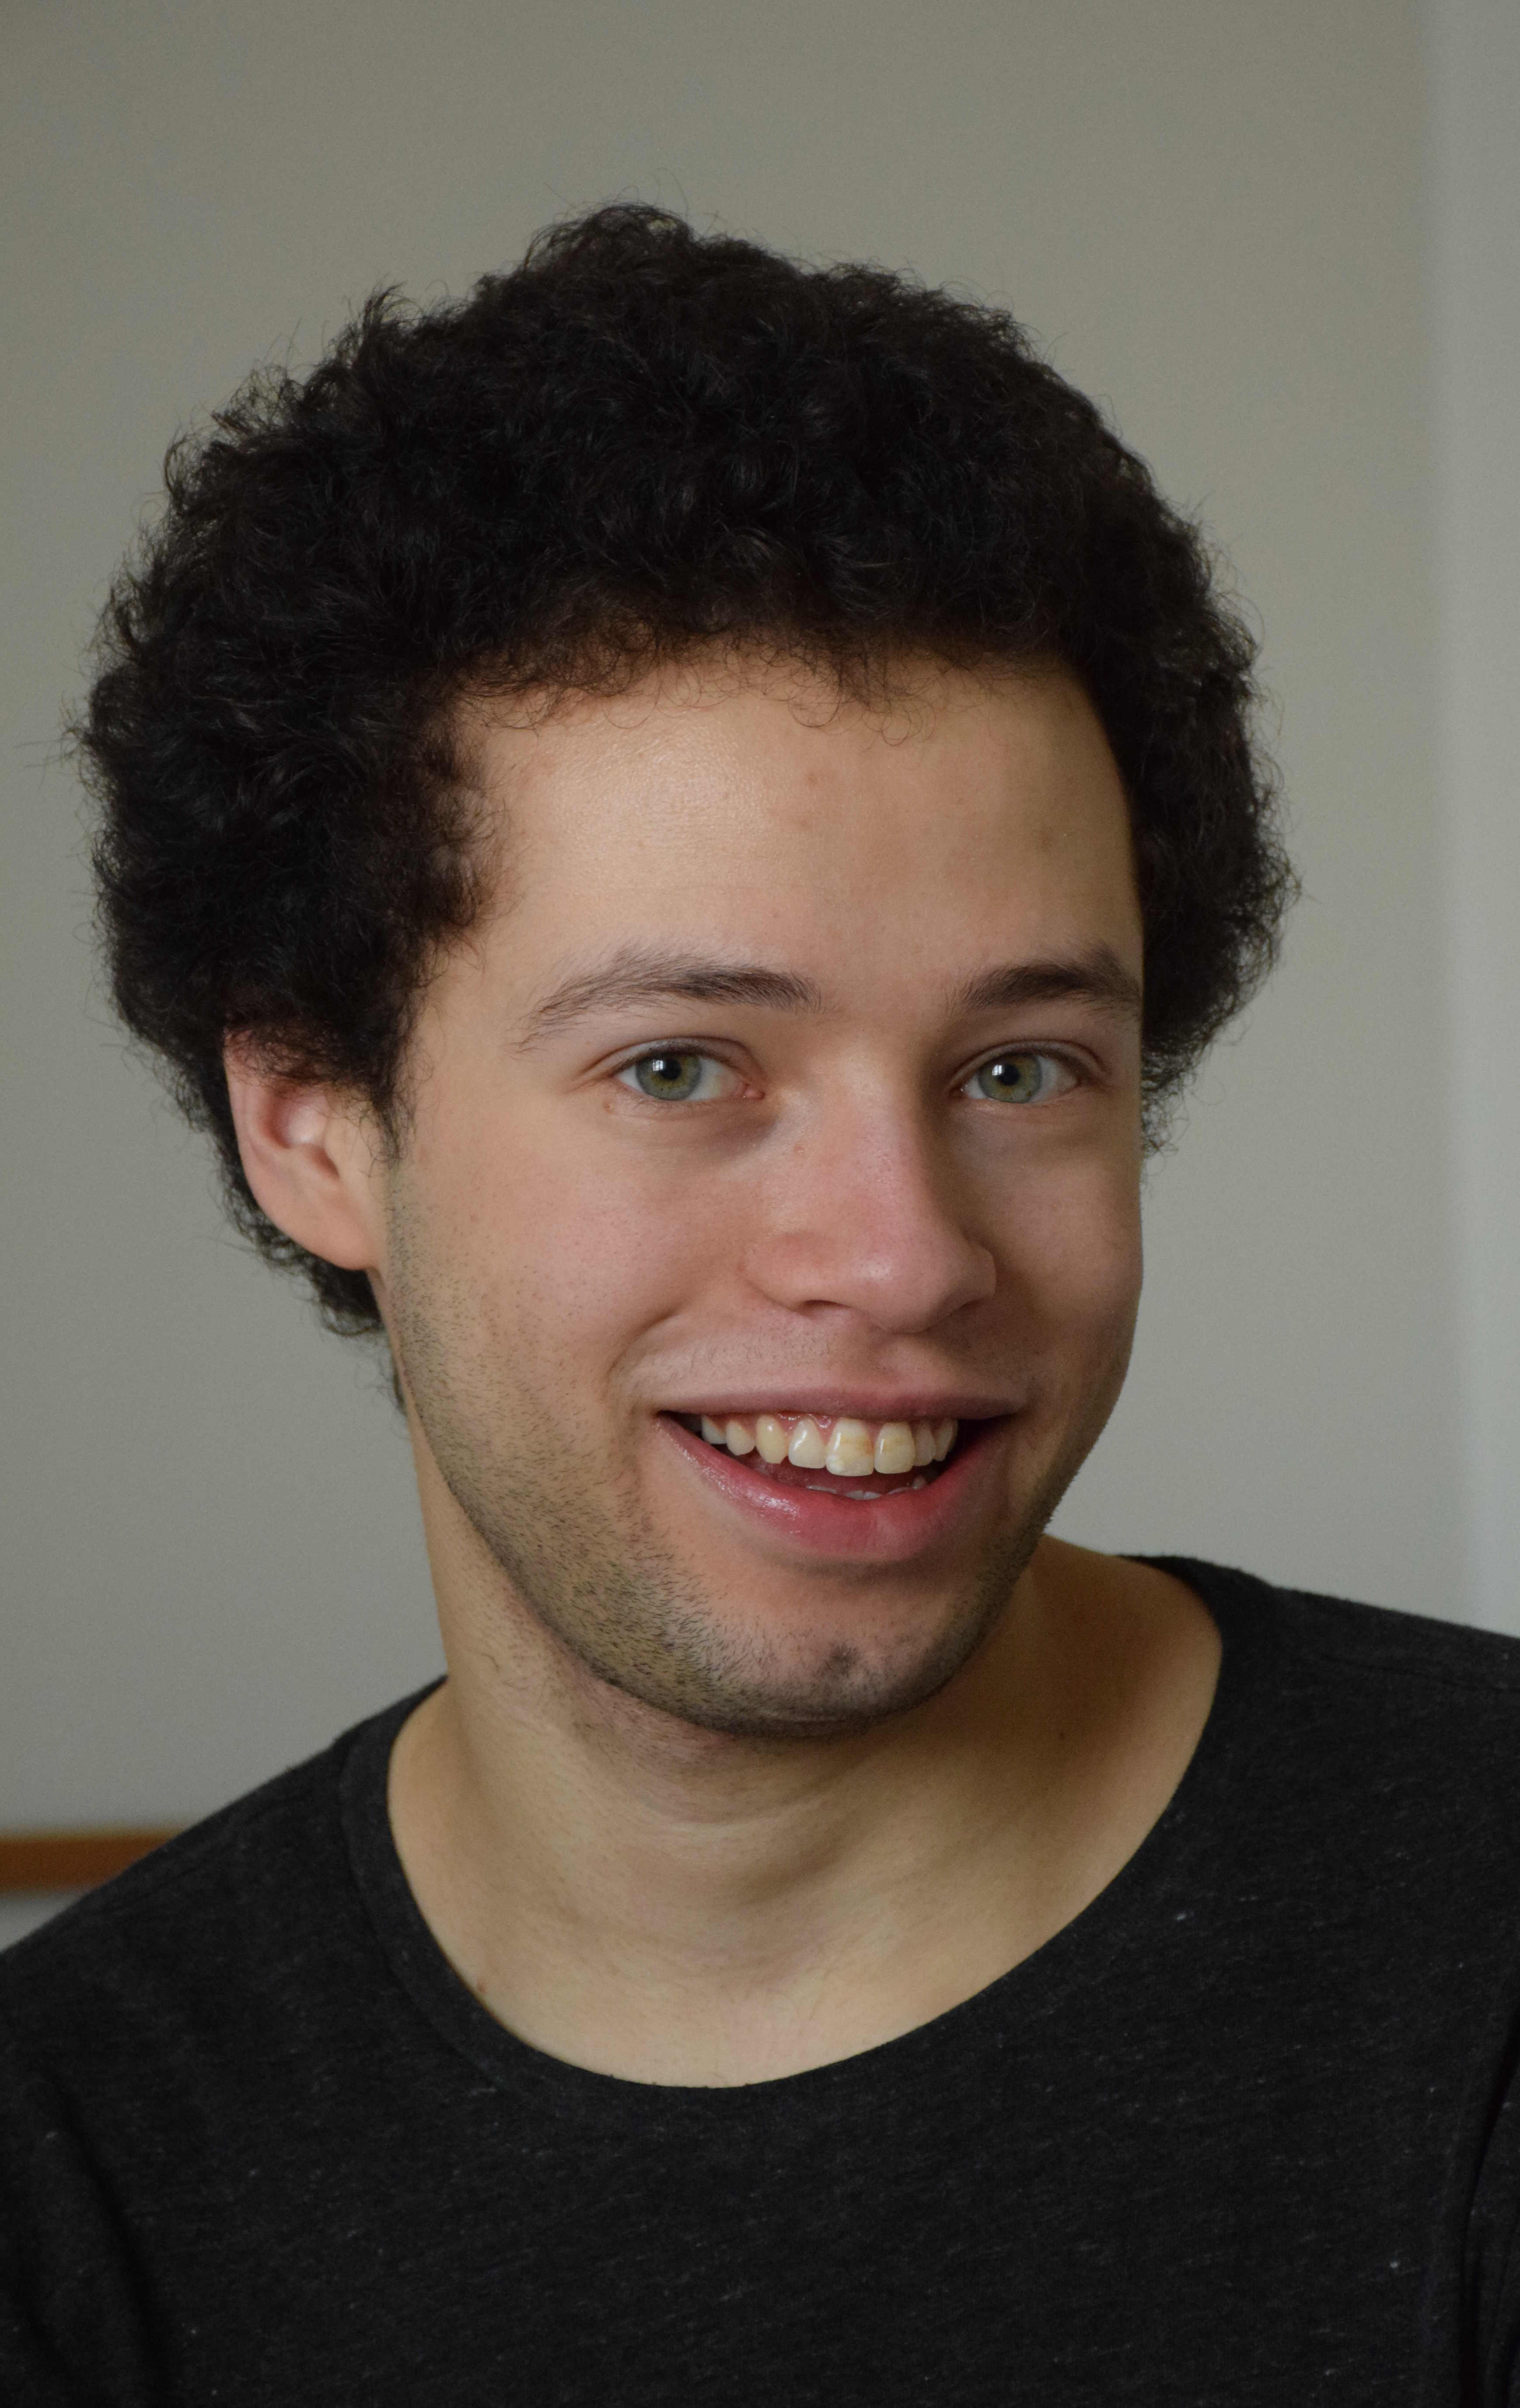
\includegraphics[width=3cm]{bild.jpeg}\\[\bigskipamount]
	% TODO hitta en bättre bild
}
\posttitle{\end{center}}
\title{
\huge{CV - Malcolm Vigren}\vspace{-3ex}}
\date{\today}
\begin{document}
	\maketitle
\underline{Malcolm} John Shubi Vigren, 19950127-0970

Batterigatan 9

587 50 Linköping

Email: \underline{trekommafem2 \textbf{at} gmail.com}

Phone: 072-534 16 81

\section*{Experience}
\noindent\begin{tabular}{@{}l p{13cm}}

\textbf{2019 -} & Ongoing Masters Thesis at Veoneer in Linkoping, on the topic
    of holistic lane detection using deep learning. \\

\textbf{2018} & Lab assistant and seminar teacher in the fall in the
    introductory Python course TDDE23/24 at Linkoping University. \\

\textbf{2018} & Part-time and summer job at Veoneer in Linkoping, from April to
    August. Worked in the team responsible for data management. \\

\textbf{2017} & Lab assistant and seminar teacher in the fall in the
    introductory Python course TDDE23/24 at Linkoping University. \\

\textbf{2017} & Summer job at Autoliv in Linkoping. Developed tools for
    processing data and storing them in a database using C\# and Microsoft SQL
    Server. \\

\textbf{2016} & Summer job at Autoliv in Linkoping. Developed tools for
    performing regression tests in Python and C\#.\\

\textbf{2015 - 2016:} & Part-time work at ICA Supermarket Eneby in Norrkoping. \\

\textbf{2013:} & Created an animated promotional video for SundaHus.
\\

\textbf{2012 - 2015:} & Part-time work at Hemköp Ljungsbrohallen in Ljungsbro. \\

	\end{tabular}

\section*{Education}
\noindent\begin{tabular}{@{}l p{11cm}}
	\textbf{Higher Education:} & \textit{Linkoping University} - Masters of
    Science in Computer Engineering 300hp, specializing in image processing and
    machine learning - Started, since fall 2014 \\

	\textbf{High School:} & \textit{Berzeliusskolan} - Teknikvetenskap -
	Finished, graduated in 2014 \\

	\textbf{Elementary School:} & \textit{The International English School in Linkoping},
	year 6-9 \\

	\textbf{Elementary School:} & \textit{Brunnbyskolan}, year 1-5 \\
	\end{tabular}

\section*{Programming skills}
Extensive knowledge in C, C\#, C++, Java, Python, VHDL, Matlab, JavaScript
and assembly language. Basic knowledge in ASP.NET, HTML, Haskell, BASH script,
CoffeeScript, Ruby On Rails and Rust.

Extensive knowledge in Git, VIM, LaTeX, and the deep learning libraries PyTorch
and Keras.

Extensive knowledge in image processing, computer vision and deep learning.

\section*{Language}
Fluent in written and spoken Swedish and English. High school level knowledge
in German.

\section*{Profile and interests}
I'm systematic, thorough and a quick learner. My main interests are
programming, science, technology, mathematics, computers, engines and cars. I
spend a large part of my spare time programming hobby projects.

\section*{Miscellaneous remarks}

Driver's license (AM and B).

Participated in the winning team in one of the competitions at LiTHe Kods
Jubileumshack in February 2016, in which an algorithm for furnishing and
visualizing a room was to be developed over night.

Received 1000 kr from Berzeliusskolan at graduation for my high grades.

\end{document}
